\chapter[Umgebungswahrnehmung mit Punktwolken (Kopp)]{Umgebungswahrnehmung mit Punktwolken}

Üblicherweise wird die Struktur einer Umgebung, die von Sensoren durch Ent\-fern\-ungs\-mess\-ung\-en abgetastet wird, von dreidimensionalen Punktwolken repräsentiert. Sie setzen sich aus einer Menge von Punkten zusammen. Jeder Punkt beschreibt die Lage eines Messpunktes im Raum. Ein Messpunkt stellt dabei einen Punkt dar, an dem die Entfernungsmessung auf Materie trifft. Die Punktwolke stellt damit eine dreidimensionale Vermessung des Raumes dar, aus der direkt Maße in x-,y- und z-Richtung gewonnen werden können. 

\begin{figure}
    \centering
    \includegraphics[width=\linewidth]{Bilder/PCS.png}
    \caption{Beispiel zum Vergleich der Abbildung eines Objektes (a) als zweidimensionales Farbbild und als dreidimensionale Punktwolke (b) ohne und (c) mit Farbwerten}
    \label{fig:pc}
\end{figure}

Abbildung \ref{fig:pc} zeigt exemplarisch eine dreidimensionale Punktwolke einer Pflanze. In (a) ist als Referenz die zweidimensionale Abbildung als Farbbild zu sehen. In (b) wird die zugehörige dreidimensionale Punktwolke gezeigt, die nur die Tiefeninformtionen enthält. Eine Punktwolke kann jedoch auch zusätzliche Attribute abspeichern, wie beispielsweise Farbwerte oder Messgenauigkeiten. Abbildung \ref{fig:pc} (c) zeigt die Punktwolke mit den zugehörigen Farbwerten jedes Punktes. 

Jeder Punkt wird durch x-y-z-Koordinaten in einem festen kartesischen Koordinatensystem beschrieben. Üblicherweise liegt der Ursprung dieses Koordinatensystems im Sensor, der die Punktwolke generiert. 

Bei großen Punktwolken, wie beispielsweise der Aufnahme einer ganzen Wohnung, stellen dreidimensionale Punktwolken große Datenmengen dar. Je größer die Punktwolke ist, desto höher sind die Anforderungen an die Rechenkapazität zur Gewinnung von Informationen. Außerdem wird viel Speicherplatz benötigt. Daher gibt es eine Menge verschiedener Algorithmen zur Verarbeitung von Punktwolken, beispielsweise für die Komprimierung oder zur effizienten Herausarbeitung von Informationen wie Um\-ge\-bungs\-merk\-male oder Objekte. Die gängigsten Algorithmen sind in verschiedenen Bibliotheken, wie beispielsweise der Point Cloud Library\footnote{\url{http://www.pointclouds.org/}} (PCL) verfügbar. Punktwolken sowie die zugehörigen Verarbeitungsalgorithmen sind nicht auf drei Dimensionen beschränkt. Mit Hilfe von Punktwolken können auch höherdimensionale Daten abgebildet werden. So finden sie beispielsweise häufig Anwendung in der Statistik zur graphischen Darstellung von Daten. 

Im Folgenden werden zunächst die gängigsten Sensoren und ihre Funktionsweise zur dreidimensionalen Umgebungswahrnehmung vorgestellt. Anschließend werden verschiedene Verfahren zur Verarbeitung von Punktwolken erklärt, die im ver\-wen\-det\-en SLAM-Algorithmus angewendet werden. Abschließend wird die PCL kurz vor\-ge\-stellt.

\section[Sensorik zur Umgebungswahrnehmung (Kopp)]{Sensorik zur Umgebungswahrnehmung}

Menschen orientieren sich in ihrer Umgebung mit Hilfe ihrer Augen, Ohren, Nase und den empfindlichen Rezeptoren der Haut. Ebenso benötigen Roboter für die jeweilige Umgebung angepasste Sensorik, um ihre Umgebung wahrzunehmen und sich sicher orientieren zu können. Diese Sensoren können im Allgemeinen in zwei Gruppen eingeteilt werden, die propriozeptiven Sensoren und die exterozeptiven Sensoren.

Die propriozeptiven Sensoren messen intern Zustände des Roboters aus denen z.B. die Odometrie bestimmt werden kann. Dazu zählen z.B. Drehgeber, die die Rad\-um\-dreh\-ung\-en detektieren, sowie Lagesensoren, wie beispielsweise ein Gyroskop. Auch Spannungssensoren, zum Messen des Ladezustands der Batterie, zählen z.B. zu dieser Gruppe.

Exterozeptive Sensoren messen externe Zustände und werden für die Wahr\-nehm\-ung der Umgebung genutzt. Dies können unter anderem Kameras, RGB-D Kameras, La\-ser\-sen\-sor\-en, Radar oder Ultraschallsensoren sein. Es wird zwischen passiven und aktiven Sensoren unterschieden. Eine Kamera stellt beispielsweise einen passiven Sensor dar, da sie nur die Energie der Umgebung in Form von Licht nutzt. Aktive Sensoren dagegen senden Energie, wie z.B. Laserstrahlen oder Schall, aus, um dann die Antwort z.B. in Form von reflektiertem Licht oder Ton auszuwerten. Daraus lassen sich wiederum der Abstand und die Richtung zu einem Objekt bestimmen.

\subsection[LiDAR (Kopp)]{LiDAR}

LiDAR steht für Light Detection and Ranging und bezeichnet ein Messverfahren, das oft für die Ortung und Entfernungsmessung von Objekten im Raum genutzt wird. Ähnlich wie beim Radar, erfolgt die Messung dabei, indem die Reflexion eines ausgesendeten Signals gemessen wird. Hierfür wird ein Lichtstrahl ausgesendet. Da Festkörper Licht reflektieren, wird die Zeit gemessen bis der reflektierte Lichtstrahl empfangen wird. Anhand der bekannten Lichtgeschwindigkeit von etwa 300.000 $ \dfrac{km}{s} $, kann die Entfernung zu dem reflektierenden Objekt bestimmt werden. Diese Methode der Entfernungsmessung wird auch Time of Flight (TOF) genannt.

%Anhand der Zeit, die dabei zwischen dem Aussenden und Empfangen gemessen wird, kann, mithilfe der bekannten Lichtgeschwindigkeit von etwa 300.000 Kilometern pro Sekunde, die Entfernung zu dem reflektierenden Objekt bestimmt werden. Diese Methode der Entfernungsmessung wird auch Time of Flight (TOF) genannt.

Generell zeichnen sich LiDAR-Systeme gegenüber anderen Sensoren zur Umgebungswahrnehmung, wie beispielsweise Kamerasysteme, dadurch aus, dass ihre Messungen sehr viel robuster gegenüber Variationen der Umgebungsbeleuchtung und Blickwinkeländerungen sind. %Auch werden die Messungen durch Umwelteinflüsse wie Regen, Schnee oder Nebel kaum beeinflusst. 
Es können sehr hohe Reichweiten von bis zu 300 m er\-reicht werden. Im Vergleich zum verwandten Radar können viel höhere Auflösungen erzielt werden. Ein weiterer Vorteil gegenüber anderen Messverfahren ist die direkt erzeugte Punktwolke, die einer Umgebungsvermessung mit absoluten Größen entspricht. 

LiDAR-Sensoren senden in der Regel Laserlichtimpulse im ultravioletten oder infraroten Bereich aus, der für den Menschen nicht sichtbar ist. Es werden zwei- und dreidimensionale LiDAR-Sensoren unterschieden. Zudem werden diese in me\-cha\-nische, Solid-State und Hybrid Solid-State, sogenannten MEMS (micro electro mechanical) \linebreak LiDARs klassifiziert.

\afterpage{
\begin{figure}
	\centering
	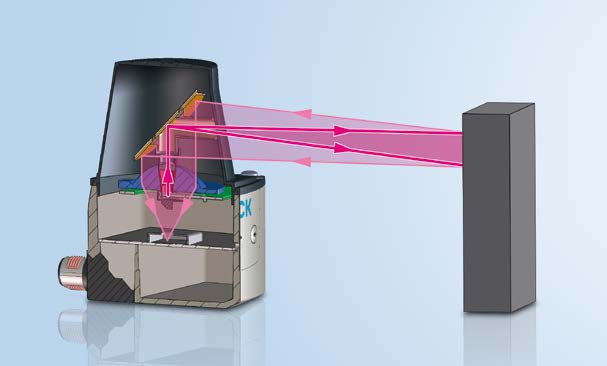
\includegraphics[width=0.55\linewidth]{Bilder/Whitepaper_LiDAR_en_IM0079963.jpg}
	\caption[Funktionsweise eines zweidimensionalen 360$^\circ$-LiDAR der Firma SICK]{Funktionsweise eines zweidimensionalen 360$^\circ$-LiDAR der Firma SICK\footnotemark}
	\label{fig:2DLaser}
\end{figure}
\footnotetext{\url{https://cdn.sick.com/media/docs/3/63/963/Whitepaper_LiDAR_en_IM0079963.PDF}, S.9}
}

\textbf{Mechanische LiDAR-Sensoren} generieren in horizontaler Ausrichtung häufig eine 360$^\circ$-Repräsentation ihrer Umgebung \cite{Weber2020}. In Abbildung \ref{fig:2DLaser} ist die Funk\-tions\-weise eines mechanischen zweidimensionalen LiDAR-Sensors dargestellt, der eine 360$^\circ$ Abbildung der Umgebung ermöglicht. Der Laserstrahl wird vertikal ausgesendet und über einen sich rotierenden Spiegel in horizontale Richtung umgelenkt. Die aus der Umgebung reflektierten Strahlen werden wieder durch den Spiegel umgelenkt und tref\-fen über eine Optik auf einen lichtempfindlichen Sensor. Über den rotierenden Spiegel wird eine schrittweise Abtastung der Umgebung erzeugt. Das Prinzip kann so er\-wei\-tert werden, dass zusätzlich eine vertikale Abtastung der Umgebung erfolgt. Dadurch wird eine dreidimensionale Vermessung erzielt. Ein Vorteil dieser Systeme ist, dass mit einem einzigen Sensor eine 360$^\circ$-Aufnahme der Umgebung erfasst werden kann. Dagegen ist ein Nachteil dieser Systeme die oft sehr große und schwere Bauweise, vor allem bei den dreidimensionalen Systemen. Außerdem wird sowohl an die Optik, als auch an die Aktorik  ein hohes Maß an Präzision gestellt. Dies macht die Systeme sehr teuer und unter Umständen wartungsaufwendig. 
 
\textbf{Solid-State Sensoren} sind in den letzten Jahren vermehrt in den Fokus der Ent\-wick\-lung gerückt \cite{FM2020}. Diese zeichnen sich im Allgemeinen durch ihre kompakte Bauweise und ihren mittlerweile vergleichsweise sehr günstigen Anschaffungspreis aus. Die halbleiterbasierte Technologie, die ohne aufwendig bewegliche Bauteile auskommt, macht sie zudem sehr robust und leicht. Nachteilig gegenüber der mechanischen Variante ist der verhältnismäßig kleine Sichtbereich. Dies kann jedoch durch die Verwendung mehrerer Sensoren in verschiedenen Ausrichtungen kompensiert werden. So können auch verschiedene Sensoren mit spezifischen Eigenschaften, wie einer hohen Reichweite in Fahrtrichtung oder einem weiten Blickwinkel im Nahbereich, dort an einem Fahrzeug kombiniert platziert werden, wo sie benötigt werden.
% Enger Blickwinkel in Ferne und breiter Blickwinkel in Nähe

\afterpage{
\begin{figure}
	\centering
	\includegraphics[width=\linewidth]{Bilder/LiDAR_Schema.png}
	\caption[Funktionsweise verschiedener Solid-State LiDAR-Sensoren]{Funktionsweise verschiedener Solid-State LiDAR-Sensoren\footnotemark}
	\label{fig:SSD_LIDAR}
\end{figure}
\footnotetext{\url{https://www.forschungsfabrik-mikroelektronik.de/de/unser-angebot/anwendungsbereiche/Transport_and_Smart_Mobility/lidar.html}}
}
 
Abbildung \ref{fig:SSD_LIDAR} zeigt die prinzipielle Funktionsweise von verschiedenen Solid-State LiDAR Technologien. Die in (a) dargestellten reinen Halbleitermodule funktionieren meist mit einem Array von Laserdioden und einem Array lichtempfindlicher Sensoren. Die Umgebung kann dabei durch eine einzige Messung erfolgen. Dies lässt eine sehr hohe Bildwiederholrate zu. Die MEMS in (b) hingegen haben bewegliche Mikrospiegel, die durch anlegen eines elektrischen Felds sehr schnell bewegt werden können. Ähnlich wie bei rein mechanischen Systemen wird die Umgebung so schrittweise abgetastet. 
  
Beide Verfahren können mit etablierten Herstellungsverfahren der Halbleiterproduktion in großen Stückzahlen vollautomatisiert hergestellt werden. Dies ermöglicht niedrige Stückpreise. Vor allem die Automobilindustrie treibt die Entwicklung der Solid-State LiDARs stark voran, da die hochauflösende Umgebungserkennung als Schlüsseltechnologie für das autonome Fahren angesehen wird. Die rein mechanischen Systeme kommen, wegen der oben aufgeführten Nachteile nicht für die Serienproduktion moderner Fahrzeuge in Frage. Auch aktuelle Top Smartphones und Tablets verfügen mittlerweile über LiDAR-Sensoren auf Basis der Solid-State Technik. Sie werden vor allem für die Verbesserung von Tiefeneffekten der Kameras, biometrische Ge\-sichts\-er\-ken\-nung und für Augmented Reality Anwendungen eingesetzt.

%
%https://www.forschungsfabrik-mikroelektronik.de/de/unser-angebot/anwendungsbereiche/Transport_and_Smart_Mobility/lidar.html
%
%https://cdn.sick.com/media/docs/3/63/963/Whitepaper_LiDAR_en_IM0079963.PDF

%\subsection{Kamera}

\subsection[RGB-D Kamera (Kopp)]{RGB-D Kamera}

RGB-D Kameras unterscheiden sich von herkömmlichen Kameras darin, dass sie zu\-sätz\-lich zum zweidimensionalen Farbbild eine Tiefeninformation registrieren können. Im Feld der mobilen Robotik hat die Technik im Gegensatz zu anderen tiefeninformationsgebenden Systemen, wie beispielsweise mechanischen LiDARs, den entscheidenden Vorteil, dass sie keine teure Kinematik mit beweglichen Bauteilen benötigen. Daher sind einige Modelle bereits für unter 200 Euro im Handel erhältlich. Auch sind viele Modelle äußerst kompakt und leicht. Zudem werden zusätzlich zur Tiefeninformation auch Farben erkannt und können ausgewertet werden. Ein Nachteil gegenüber LiDAR-Sensoren ist der eingeschränkte Blickwinkel einer einzelnen Kamera und die ver\-gleichs\-wei\-se geringe zuverlässige Reichweite von etwa 20 m. Ihre Eigenschaften machen sie zu einem beliebten Sensorsystem für mobile Roboter. Einsatzfelder sind häufig indoor-Anwedungen, bei denen Reichweiten bis zu 10 m von Interesse sind. Die Ausgabe ist je nach Kamera neben dem Farbbild eine Punktwolke oder ein Tiefenbild. Es gibt jedoch Verfahren mit denen beide Ausgaben der Tiefeninformationen ineinander überführt werden können. Außerdem kann das Farbbild mit der Punktwolke registriert werden. Dadaurch entsteht eine farbige Punktwolke.

Es gibt im Allgemeinen vier Arten wie die Tiefeinformation bei RGB-D-Kameras ermittelt werden kann. Diese sind auf Abbildung \ref{fig:RGBD_Kameras} dargestellt. 

\begin{figure}
	\centering
	\includegraphics[width=\linewidth]{Bilder/RGBD_Kameras.png}
	\caption{Darstellung der verschiedenen Techniken zur Erzeugung von Tiefeinformationen bei RGB-D Kameras}
	\label{fig:RGBD_Kameras}
\end{figure}
 
\textbf{Time of Flight Kameras} zählen zu den aktiven Sensoren, da sie die Umgebung durch aktiv ausgestrahltes Licht abtasten \cite{Shao2014}. Das Funktionsprinzip zur Gewinnung der Tiefeninformation ist gleich wie bei den Solid-State LiDARs. Abbildung \ref{fig:RGBD_Kameras} (a) zeigt den Aufbau des Systems. Es besteht aus einer Kamera und einer Lichtquelle. Die Lichtquelle sendet einen kurzen Lichtimpuls aus. Die Lichtstrahlen werden von der Umgebung reflektiert und fallen auf einen lichtempfindlichen Sensor, die Kamera, zurück. Aus der bekannten Lichtgeschwindigkeit und der Zeit, die das Licht vom Aussenden bis es auf die Kamera fällt benötigt, lässt sich so für jeden Bildpunkt eine Entfernung berechnen. Das Licht befindet sich meist im für Menschen nicht sichtbaren infraroten Bereich. Die Vorteile dieses Typs sind vor allem die hohen Bildwiederholraten von mehreren 100 Bildern pro Sekunde sowie ihr simpler Aufbau.
 
\textbf{Structured Light} wird eine Technik genannt, bei der ein Projektor ein Infrarotmuster über die Szene legt \cite{Shao2014}. Als Muster werden oft pseudo-zufällige Anordnungen von Punkten verwendet. Abbildung \ref{fig:SLBsp} zeigt ein Beispiel eines solchen Punktmusters. Durch einen Kamerasensor, der im Infrarotbereich arbeitet, wird diese Projektion wahrgenommen. Dem verarbeitenden Algorithmus ist der Abstand des Projektors zur Kamera sowie das ausgesendete Muster bekannt. Anhand des veränderten Abstands der Punkte im Bild kann durch Triangulation der Abstand dieser Punkte zur Kamera berechnet werden. Der Aufbau des Kamerasystems ist auf Abbildung \ref{fig:RGBD_Kameras} (b) dargestellt. Ein Nachteil des Systems ist die Fehleranfälligkeit durch andere Lichtquellen im gleichen Wellenbereich, wie beispielsweise das Sonnenlicht. 

\begin{figure}[htb]
	\centering
	\begin{minipage}[t]{0.45\linewidth}
		\centering
		\includegraphics[width=\linewidth]{Bilder/infrared.png}
		\caption{Beispiel eines pseudo-zufälligen Punktmusters einer Structured Light Kamera}
		\label{fig:SLBsp}
	\end{minipage}
	\hfill
	\begin {minipage}[t]{0.45\linewidth}
		\centering
		\includegraphics[width=\linewidth]{Bilder/Stereoskopie.png}
		\caption{Ermittlung der Tiefeinformation anhand der Disparität korrespondierender Bildpunkte }
		\label{fig:Stereoskopie}
	\end{minipage}
\end{figure}
 
\textbf{Passive Stereoskopie} funktioniert im Gegensatz zu den zuvor vorgestellten Verfahren ohne das Aussenden von Signalen \cite{Modrow2008}. Es handelt sich daher um ein passives Verfahren. Wie auf Abbildung \ref{fig:RGBD_Kameras} (c) zu sehen ist, werden zwei Kameras benötigt, die eine Szene aus verschiedenen Perspektiven aufnehmen. Abbildung \ref{fig:Stereoskopie} zeigt das Funktionsprinzip. Um eine Tiefeninformation zu erhalten, werden zunächst in jedem Bild Keypoints extrahiert. Diese werden verglichen, um Korrespondenzen in beiden Bildern zu finden. In der Abbildung symbolisiert das Kreuz einen Keypoint, der eine Kor\-re\-spon\-denz zwischen beiden Bildern darstellt. Anschließend wird die Disparität, die dem Unterschied der x-Koordinaten der korrespondieren Punkte entspricht, ermittelt. Da der genaue Abstand zwischen den Kameras bekannt ist, kann mit Hilfe der Dis\-pa\-ri\-tät die Entfernung jedes Keypoints zur Kamera berechnet werden.

Die passive Stereoskopie ist im Gegensatz zu den beiden vorgestellten aktiven Verfahren nicht anfällig für Fehler durch Sonnenlicht. Außerdem sind prinzipiell höhere Reichweiten realisierbar wie bei aktiven Ansätzen. Jedoch kann die Extraktion von eindeutig identifizierbaren Keypoins, beispielsweise auf einfarbigen strukturlosen Flächen, eine nicht leicht zu lösende Aufgabe darstellen, die nicht immer zu robusten Ergebnissen führt. 

\textbf{Aktive Stereoskopie} verwendet einen hybriden Ansatz, bei dem eine Kombination aus Structured Light und Stereoskopie verwendet wird \cite{Modrow2008}. Die Korrespondenzsuche wird deutlich vereinfacht, da mit Hilfe des Structured Light Ansatzes Keypoints in die Umgebung projiziert werden. Die Tiefeninformationen werden anschließend wie bei der passiven Stereoskopie ermittelt. Der Vorteil ist, dass Fehler durch  störendes Licht ausgeglichen werden können, indem auf die passive Stereoskopie zurückgegriffen wird. Außerdem können auch Entfernungen zu Oberflächen, auf denen Keypoints nur schwer oder gar nicht extrahiert werden können, bestimmt werden. 


\section[Registrierung (Kopp)]{Registrierung}

Wenn ein oder mehrere tiefeninformationsgebende Sensoren ein Objekt oder eine Umgebung aus verschiedenen Blickwinkeln aufnehmen, müssen die Punktwolken der einzelnen Messungen zusammengefügt werden. Dies wird Registrierung genannt. Da jede Punktwolke ein eigenes Koordinatensystem hat, müssen die einzelnen Punktwolken in ein gemeinsames Koordinatensystem übertragen werden. 

\subsection[Problemdefinition (Kopp)]{Problemdefinition}

Die Registrierung wird auch in der Bildverarbeitung verwendet. Beispiele für die Anwendung von Bildregistrierung sind Panoramaaufnahmen oder die dreidimensionale Rekonstruktion von Objekten. Hierbei werden mehrere Bilder einer Szene oder eines Objektes aus verschiedenen Perspektiven aufgenommen, um einen größeren Blickwinkel abzudecken oder eine dreidimensionale Abbildung eines Objektes zu erhalten. 

Ist die genaue Position des Sensors für jede Aufnahme bekannt, kann die Re\-gis\-trie\-rung auf Basis der relativen Lage der Aufnahmen zueinander durchgeführt werden. Die Positionen der Sensoren müssen dafür jedoch sehr genau gegeben sein, da bereits geringe Abweichungen dazu führen, dass die Aufnahmen nicht sinnvoll zusammengefügt werden. Eine so genaue Position der Sensoren ist nur mit hohem Aufwand zu ermitteln und in der Regel bei Anwendungen mobiler Roboter nicht gegeben. 

Es gibt verschiedene Ansätze die Registrierung auf Basis der Punktwolken durch\-zu\-füh\-ren. Um diese zusammenfügen zu können, müssen die Aufnahmen einer Szene sich in einem gewissen Bereich überlappen. Die Punktwolken werden dann so zusammengefügt, dass sie im überlappenden Bereich übereinstimmen. 

Es wird ein Koordinatensystem bestimmt, in das alle Punktwolken eingefügt werden. Häufig wird das Koordinatensystem einer der Punktwolken verwendet, die dann die Referenzpunktwolke bildet. Alle anderen Punktwolken werden an diese angefügt. Das Ergebnis der Registrierung ist die Transformation einer Punktwolke in das Re\-fe\-renz\-ko\-or\-di\-na\-ten\-sys\-tem, die die Punktwolken am besten in Übereinstimmung bringt. Diese Transformation setzt sich aus einer Rotation und einer Translation der Punktwolke zusammen. 

Abbildung \ref{fig:Registrierung} zeigt ein Beispiel zur Registrierung mehrerer Punkt\-wol\-ken. Die Punkt\-wol\-ken bilden die Struktur eines Raumes ab, der aus sechs verschiedenen Blickwinkeln aufgenommen ist. Die einzelnen Punktwolken überlappen sich teilweise. Die überlappenden Bereiche werden durch die Registrierung so übereinander gelegt, dass eine  Punktwolke entsteht, die die Umgebung abbildet. 

\afterpage{
\begin{figure}
    \centering
    \includegraphics[width=\linewidth]{Bilder/PCS_registriert.png}
    \caption[Beispiel zur Registrierung von Punktwolken]{Beispiel zur Registrierung von Punktwolken\footnotemark}
    \label{fig:Registrierung}
\end{figure}
\footnotetext{\url{https://pcl-tutorials.readthedocs.io/en/latest/registration_api.html\#registration-api}}
}

Im Kontext der mobilen Robotik wird die Registrierung von Punktwolken häufig verwendet, um die Posenschätzung eines Roboters zu erhalten oder zu verbessern. Die Posenschätzung wird auf Basis von Odometriedaten 
%oder Lokalisierungsmethoden 
getroffen, auf die in Kapitel \ref{sec:Lokalisierung} genauer eingegangen wird. Es wird dann von Scan Matching gesprochen. 

Abbildung \ref{fig:ScanMatching} zeigt eine typische SLAM-Anwendung. Eine unbekannte Umgebung wird durch einen mobilen Roboter erkundet, der ohne Informationen über seine Pose eine Karte der Umgebung erstellt. Die linke Abbildung zeigt die Karte, die nur anhand der Odometriedaten entsteht. Die rechte Abbildung zeigt die Karte, die mit Odometriedaten erstellt wird, die durch Scan Matching verbessert werden. Es ist deutlich zu sehen, dass die Schätzung der Roboterpose mit Unterstützung von Scan Matching zu besseren Resultaten führt. 
% http://kos.informatik.uni-osnabrueck.de/download/diplom/diplom.html ??

\afterpage{
\begin{figure}
    \centering
    \includegraphics[width=\linewidth]{Bilder/ScanMatching.png}
    \caption[Beispiel für die Verbesserung der Odometrie durch Scan Matching bei einer SLAM-Anwendung]{Beispiel für die Verbesserung der Odometrie durch Scan Matching bei einer SLAM-Anwendung\footnotemark}
    \label{fig:ScanMatching}
\end{figure}
\footnotetext{\url{http://ais.informatik.uni-freiburg.de/teaching/ws12/mapping/pdf/slam12-scanmatching-mini.pdf}, S.7}
}

%Die Bilder müssen sich für eine Registrierung teilweise überlappen. In diesen bereichen werden markante Punkte gesucht, dieeindeutig in beiden Bildern als Korrepsondenz identifiziert werden können. Die Bilder werden dann so aneinandergehangen, dass diese markanten Punkte aufeinander gelegt werden. 

Für die Registrierung von Punktwolken gibt es verschiedene Ansätze. Merkmal-basierte Ansätze, deren Prinzip auch in der Bildverarbeitung angewendet werden, extrahieren markante  Stellen oder Bereiche aus den Punktwolken, wie beispielsweise Punkte oder Linien \cite{Simon1994}. Anschließend werden Korrespondenzen zwischen gleichen Merkmalen in den Punktwolken gesucht. Aus den Positionen der Korrespondenzen wird die Transformation berechnet, anhand der die Punktwolken in ein gemeinsames Koordinatensystem übertragen werden können. 
% Allerdings kann es schwierig sein zuverlässig eindeutig identifizierbare Merkmale in Punktwolken zu finden. Außerdem ist die Merkmalsextraktion rechenintensiv. 

Die Registrierung kann auch als Optimierungsproblem betrachtet werden. Ein häufig verwendeter Algorithmus hierfür ist der Iterative Closest Points (ICP) Algorithmus, der im Folgenden beschrieben wird. 

\subsection[ICP (Kopp)]{ICP}

Häufig wird der ICP-Algorithmus für die Registrierung von Punktwolken verwendet. Das Ziel ist es eine Transformation zu ermitteln, die die Punktwolken mit der höchs\-ten Übereinstimmung zusammenfügt. Zu Beginn wird eine initiale Transformation geschätzt, die iterativ angepasst wird. Als Gütekriterium einer Transformation wird eine Fehlerfunktion verwendet, die minimiert wird. 
%Diese Transformation wird iterativ angenähert, indem in jedem Schritt eine neue Transformation bestimmt wird.

Es gibt viele verschiedene Variationen des ICP-Algorithmus, die sich beispielsweise in der Bestimmung der initialen Transformation oder anhand der verwendeten Fehlerfunktion unterscheiden. Ansätze für die Bestimmung der initialen Transformation sind z.B. über die Odometriedaten eines mobilen Roboters oder über eine Extraktion von korrespondierenden Merkmalen in den Punktwolken.

Alle Varianten des ICP-Algorithmus basieren jedoch auf dem gleichen Funk\-tions\-prin\-zip \cite{Rusinkiewicz2001}. 
Gegeben sind zwei Punktwolken $ P $ und $ M $, die in ein gemeinsames Koordinatensystem registriert werden sollen. Das Ziel ist eine Menge kor\-res\-pon\-die\-ren\-der Punkte in beiden Punktwolken zu finden anhand derer die gesuchte Transformation berechnet werden kann. Es wird angenommen, dass die Korrespondenz eines Punktes $ m_i \in M $ der Punkt $ p_j \in P $ ist, zu dem der euklidische Abstand minimal ist. 

\floatname{algorithm}{Algorithmus}
\begin{algorithm}
	\caption{Iterative Closest Points mit gegebenen Punktwolken $ M $ und $ P $.}
	\label{ICP}
	\begin{algorithmic}[1]
		\Function{ITERATIVECLOSESTPOINTS}{$ M,P $}
			\While{$ E  > \tau $}
				\State Berechnung der nächsten Punkte
				\State Berechnung der Transformation
				\State Anwendung der Transformation $ R,t $
				\State Berechnung des Fehlers $ E $
			\EndWhile
			\State \Return{$ R,t $}
		\EndFunction
	\end{algorithmic}
\end{algorithm}

Algorithmus \ref{ICP} zeigt den Ablauf des Grundprinzips, auf das alle Varianten des ICP-Algorithmus basieren. Zunächst wird in einer oder beiden Punktwolken eine bestimmte Menge von $ N_p $ Punkten ausgewählt, in denen die nächstgelegenen Punkte ermittelt werden. 
%Zunächst wird in einer oder beiden Punktwolken eine bestimmte Menge von $ N_p $ Punkten ausgewählt, in denen die nächstgelegenen Punkte ermittelt werden.
Basierend auf den ausgewählten korrespondierenden Punktpaaren wird die gesuchte Transformation zwischen den Punktwolken berechnet. Anschließend werden die Punktwolken anhand dieser Transformation registriert. Mit Hilfe der Fehlerfunktion wird die Güte der Transformation bestimmt.Hierfür wird beispielsweise der mittelere quadratische Fehler $ E $ aller Abstände zwischen allen Punktpaaren verwendet: 

\begin{align}
	E = \sum_i(Rp_i+t-m_i)^2
\end{align}

Dies wird solange wiederholt, bis der Fehler unter einen vorgegebenen Schwellwert $ \tau $ fällt. Dadurch wird die Transformation iterativ verbessert. 

%Werden zwei Punktwolken in ein gemeinsames Koordinatensystem registriert, werden zunächst in einer oder beiden Punktwolken eine bestimmte Menge von Punkten ausgewählt. Hierbei wird angenommen, dass die am nächsten gelegenen Punkte beider Punktwolken korrespondieren. Die Korrespondenzen werden über den euklidischen Abstand bestimmt. Es gibt verschiedene Methoden diese Korrespondenzen zu finden, beispielsweise über k-d Bäume, auf die in Kapitel ... näher eingegangen wird. Anschließend werden Paare korrespondierender Punkte in beiden Punktwolken gesucht. Bei manchen Formen des ICP-Algorithmus werden die einzelnen Punktpaare gewichtet oder einzelne Punktpaare basierend auf bestimmten Kriterien verworfen.


\section[Segmentierung (Schmelzer)]{Segmentierung}

Punktwolken setzen sich aus einer Menge von Punkten zusammen. Um aus dieser Punktmenge Informationen zu gewinnen, müssen Merkmale herausgearbeitet werden, die die vorliegende Punktwolke beschreiben. Hierfür gibt es verschiedene Ansätze.
%, über die in Kapitel \ref{Merkmale} ein Überblick gegeben wird. 
Die Basis einiger Verfahren zur Merkmalsextraktion aus Punktwolken bildet die Segmentierung. Hierbei werden aus den Punkten Gruppen zusammengehöriger Informationen herausgearbeitet. Die Segmentierung wird beispielsweise bei der Objekterkennung verwendet, um die Punkte zusammenzufassen, die gemeinsam  ein Objekt bilden. 

Durch die Zerlegung einer großen in mehrere kleinere Punktwolken, sogenannte Segmente, ergeben sich einige Vorteile in der Weiterverarbeitung. So lassen sich Algorithmen effizienter anwenden, da die Verarbeitung von kleineren Punktwolken schneller ist. Außerdem können die Segmente auch parallel weiterverarbeitet werden. Die Punkt\-wol\-ke kann auch gefiltert werden, sodass in der Weiterverarbeitung nur relevante Segmente verwendet werden. Wenn beispielsweise verschiedenen Objekte auf einem Tisch erkannt werden sollen, könnte die Punktwolke so gefiltert werden, dass das Segment der Tischoberfläche weg fällt. Zusätzlich wird weniger Speicherplatz benötigt, wenn z.B. Rauschen reduziert wird durch das Löschen von Punkten, die keinem Segment zugewiesen wurden. 

Die Segmentierung wird nicht nur zur Verarbeitung von Punktwolken eingesetzt, sondern ist auch ein Teilgebiet der  Bildverarbeitung. Hier wird sie ebenfalls als Vorstufe der Merkmalsextraktion verwendet. Bei der Segmentierung von Bildern werden teilweise ähnliche Verfahren verwendet wie bei der Segmentierung von Punktwolken. 

\subsection[Segmentierung in der Bildverarbeitung (Schmelzer)]{Segmentierung in der Bildverarbeitung}
%https://link.springer.com/content/pdf/10.1007%2F978-3-642-04952-1.pdf

In der Bildverarbeitung werden Bilder bei der Segmentierung in Regionen unterteilt, indem die Pixel anhand vorgegebener Kriterien verschiedenen Gruppen zugeordnet werden. Die Anzahl der sich so ergebenden Regionen ist nicht fest vorgegeben, sondern abhängig vom zugrundeliegenden Bild und des verwendeten Verfahrens. Sie wird beispielsweise als Vorstufe der Objekterkennung eingesetzt, um Objekte vom Hintergrund zu separieren. 

Für die Segmentierung gibt es verschiedene Ansätze bei denen im wesentlichen Pixel-, Kanten- und Regionen-basierte Verfahren unterschieden werden.
%Die Aufteilung eines Bildes in verschiedene Regionen kann auf Basis eines Schwellwerts für die Pixelwerte vorgenommen werden oder durch das Erkennen von Kanten. Eine weitere Methoden bildet das Region Growing  , die die Kriterien definieren anhand derer das Bild unterteilt wird.  

\subsubsection[Pixel-basierte Segmentierung (Schmelzer)]{Pixel-basierte Segmentierung}

Bei der Pixel-basierten Segmentierung werden Bildregionen anhand der  einzelnen Pi\-xel\-wer\-te, die den Helligkeitswerten bei Graustufenbildern entsprechen, unterschieden \cite{Jaehne2012}. Es wird jeder einzelne Pixel geprüft, ob sein Wert einen vorgegeben Grenzwert übersteigt und  entsprechend einer Gruppe zugewiesen. Es werden also die hellen und dunklen Bildbereiche unterschiedenen. Dadurch bilden sich zwei Bild\-be\-rei\-che heraus. Die Güte des Verfahren ist abhängig von der Wahl des  Grenzwerts, der anhand des Histogramms der Grauwerte eines Bildes gewählt wird. 

Abbildung \ref{fig:seg2d} zeigt ein Beispiel anhand des Bildes aus Abbildung \ref{fig:pc}. In (a) ist das Ausgangsbild zu sehen, das in ein Graustufenbild umgewandelt wurde. Anschließend wird es anhand der Intensitätswerte in zwei Bildbereiche unterteilt. In (b) ist das zugehörige segmentierte Bild dargestellt. Das Bild zeigt, dass das Verfahren abhängig von der Homogenität der Bildbereiche ist. Bei nicht homogenen Hintergründen und Objekten mit verschiedenen Helligkeitswerten verschmelzen durch die verschiedenen Helligkeitsstufen die Grenzen zwischen diesen und es kommt zu Löchern in den Bildregionen. Eine eindeutige Trennung eines Objektes vom Hintergrund ist dadurch nur in bestimmten Fällen möglich, beispielsweise bei der Herausarbeitung von Buchstaben oder Ziffern. 

Es handelt sich um ein simples Verfahren, das nur wenig Rechenleistung benötigt. Allerdings sind die Anwendungsbreiche eingeschränkt, da nur gute Ergebnisse erzielt werden können, wenn die verschiedenen Bildbereiche möglichst homogen sind. Außerdem ist das Verfahren abhängig von der Beleuchtung, da diese auch in homogenen Bildbereichen zu einer Abstufung der Grauwerte führen kann. Die An\-wen\-dungs\-be\-rei\-che beschränken sich daher auf Bilder, in denen die zu trennenden Bereiche deutliche Unterschiede aufweisen und homogen sind. Zudem kann die Größe eines Objekts nicht genau bestimmt werden, da diese durch leichte Grauwertabstufungen  in Randbereichen abhängig vom gewählten Grenzwert variiert. 

\begin{figure}
    \centering
    \includegraphics[width=\linewidth]{Bilder/Segmentierung2D.png}
    \caption{Beispiele zur Segmentierung in der Bildverarbeitung anhand des Bildes in (a) basierend auf (b) einen Schwellwert und (c) durch Kantenerkennung}
    \label{fig:seg2d}
\end{figure}

\subsubsection[Kanten-basierte Segmentierung (Schmelzer)]{Kanten-basierte Segmentierung}

Kanten-basierte Segmentierungsverfahren grenzen Bildbereiche durch das Erkennen von Kanten voneinander ab  \cite{Jaehne2012}. Diese zeichnen sich in Bildern durch Diskontinuitäten in den Helligkeitswerten aus. Die Positionen von Kanten werden mit Hilfe des Grauwertgradienten ermittelt. Kanten zeigen sich in der Ableitung erster Ordnung durch Extremwerte.
% und in der Ableitung zweiter Ordnung durch einen Nulldurchgang. Daher werden Kanten durch 
Daher wird bei der Kanten-basierten Segmentierung nach lokalen Maxima im Betrag des Grauwertgradienten gesucht. Häufig werden auch Kantenverfolgungsalgorithmen eingesetzt, die die Kanten entlang eines Objekts verfolgen sobald ein lokales Maximum gefunden wird. Die sich so ergebenden verschiedenen Bild\-be\-rei\-che werden durch die Kanten voneinander getrennt. Abbildung \ref{fig:seg2d} (c) zeigt ein Beispiel zur Kantenerkennung anhand des in (a) abgebildeten Graustufenbildes. 

Die Kanten-basierte Segmentierung eignet sich im Vergleich zur Pixel-basierten Segmentierung besser für Anwendungen bei denen die Größe der segmentierten Be\-rei\-che von Bedeutung ist, da diese anhand der Kante besser bestimmt werden kann. Die Segmentierung liefert bessere Ergebnisse, je höher der Kontrast eines Objektes zum Hintergrund ist. Verschmierte Kanten mit weniger Kontrast liefern hingegen schlechtere Ergebnisse, da der Gradient in diesen Bereichen kleiner ausfällt. 

\subsubsection[Regionen-basierte Segmentierung (Schmelzer)]{Regionen-basierte Segmentierung}

Für die Regionen-basierte Segmentierung gibt es verschiedene Verfahren, wie bei\-spiels\-wei\-se das Region Growing \cite{Burger2015}. Hierbei wachsen Bildregionen schritt\-wei\-se ausgehend von einem initialen Pixel. Benachbarte Pixel werden auf Basis eines vorgegeben Homogenitätskriterium zusammengefasst. Ein Kriterium kann bei\-spiels\-wei\-se ein Grenz\-wert auf die Differenz der Grauwerte sein. Wenn das Kriterium zu einem benachbarten Pixel erfüllt ist, wird dieser Pixel zu der Region hinzugefügt. Dies wird rekursiv wiederholt indem von den hinzugefügten Pixeln auf gleiche Weise wei\-ter gewachsen wird. Eine Region ist abgeschlossen, wenn keine weiteren Pixel mehr hinzukommen, da die benachbarten Punkte das Kriterium nicht erfüllen. Anschließend kann dies für weitere initiale Pixel wiederholt werden bis alle Pixel eines Bildes einer Region zugefügt sind. 
%http://users.cs.cf.ac.uk/Dave.Marshall/Vision_lecture/node35.html
%https://link.springer.com/content/pdf/10.1007%2F978-3-642-04952-1.pdf S. 547
%https://link.springer.com/content/pdf/10.1007%2F978-3-642-04604-9.pdf .  224

Für die  Wahl der initialen Pixel gibt es verschiedene Ansätze, die zum Herausbilden unterschiedlicher Regionen führen können. Um die Segmentierung zu beschleunigen, können die Pixel vor dem Region Growing in ein regelmäßiges Gitter mit fester Kantenlänge eingefügt werden. Dadurch ergeben sich Zellen gleicher Größe, beispielsweise von 4$\times$4  Pixeln. Die Segmente wachsen dann nicht von Pixel zu Pixel, sondern von einer Gitterzelle zur anderen. Dadurch werden weniger Rekursionen benötigt, um das ganze Bild in Regionen aufzuteilen. Abhängig vom gewählten Kriterium kann es al\-ler\-dings vorkommen, dass Regionen zusammenwachsen, die eigentlich getrennt sind. Dies passiert, wenn diese nur in kleinen Bereichen, beispielsweise nur zwischen zwei Pixeln das Kriterium erfüllen. Bei Gitter-basiertem Region Growing wird dies zusätzlich von der gewählten Kantenlänge beeinflusst. 

\subsection[Segmentierung von Punktwolken (Schmelzer)]{Segmentierung von Punktwolken}

Bei der Segmentierung von Punktwolken werden diese häufig in eine Gitterstruktur mit gleichmäßigen Kantenlängen eingefügt. Die einzelnen Zellen eines Gitters werden im zweidimensionalen Raum als Pixel bezeichnet, im dreidimensionalen als Voxel. Dadurch kann die Anzahl der Punkte reduziert werden, indem die Punkte in einem Pi\-xel bzw. Voxel zusammengefasst werden. Die Segmentierungsalgorithmen können in diesen Fällen auf die einzelnen belegten Pixel bzw. Voxel angewendet werden. Außerdem werden Punktwolken dadurch in eine regelmäßige Struktur gezwungen, wie sie auch bei Bildern durch die Einteilung in Pixel gegeben ist. Zusätzlich kann Speicherkapazität gespart werden, indem die Punktwolken in effizienten Datenstrukturen ge\-spei\-chert werden, wie beispielsweise Octrees, die belegte und freie Bereiche in Voxelgittern effizient zusammenfassen.

Das Prinzip einiger Segmentierungsmethoden aus der Bildverarbeitung kann auch auf Punktwolken übertragen werden. So gibt es z.B. auch Kanten-basierte Segmentierungsverfahren. Kanten zeichnen sich in Punktwolken z.B. durch starke Richtungsänderungen der Normalenvektoren oder große Differenzen in den Schätzungen der Krümmungswerte eines Punktes aus \cite{Wilke2002}. Die Krümmung eines Punktes wird hierbei durch die Krümmung der Fläche seiner Nachbarschaft geschätzt. Auch der Normalenvektor eines Punktes wird über diese Nachbarschaft ermittelt. 

Auch das Prinzip des Region Growing kann auf Punktwolken angewendet werden. Wie in der Bildverarbeitung basiert es auf dem Zusammenwachsen benachbarter Punkte, wenn diese bestimmte Kriterien erfüllen. Eine Region ist abgeschlossen sobald keine weiteren Punkte mehr hinzukommen, da sie die Bedingungen nicht erfüllen. Region Growing Algorithmen arbeiten auf Basis der Nachbarschaft eines Punktes. Daher werden die Punktwolken häufig vor der Segmentierung in effizienten Datenstrukturen, wie $k$-d-Bäumen, gespeichert, da diese die Ermittlung der benachbarten Punkte beschleunigen. Auf $k$-d Bäume und die Suche der benachbarten Punkte in diesen wird in Kapitel \ref{sec:k-d-baum} näher eingegangen. 
% Segmentierung anhand mehrerer Punkte statt nur durch Randpunkte wie bei kanten-basierten Segmenteirungsverfahren. Zuordnung der Randpunkte kann unsicher sein bei nahe gelegenen Segmenten. Jeder innere Punkt gehört jedoch nur zu einem Segment. Dadurch ist Mehrzahal der Punkte eindeutig zurordbar

Es gibt verschiedene weitere Ansätze zur Segmentierung von Punktwolken. Im folgenden werden zwei gängige Verfahren auf Basis des Region Growings erläutert, die auch in der PCL implementiert sind. Die Zuordnung der Punkte in verschiedene Regionen wird auch als Clustering bezeichnet und die entstehenden Regionen dem\-ent\-spre\-chend als Cluster. 

%Um die Nachbarschaft jedes Punktes effizient ermitteln zu können, werden die Punktwolken häufig in eine Gitterstruktur eingefasst und anschließend in eine effiziente Datenstruktur, wie bes 

\subsubsection[Euklidisches Clustern (Schmelzer)]{Euklidisches Clustern}

Beim Region Growing durch euklidisches Clustern werden benachbarte Punkte zu ei\-ner Region zusammengefasst, deren euklidische Abstände unterhalb eines vorgegebenen maximalen Abstands liegen. 

%http://www.pointclouds.org/documentation/tutorials/cluster_extraction.php#cluster-extraction
Algorithmus \ref{euklid} zeigt den Pseudocode des in der PCL verwendeten euklidischen Clustering von Punktwolken \cite{Rusu2009}. In Zeile 2 werden leere Mengen für die Cluster $ C $ und die Punkte $ Q $, die geprüft werden müssen, ob von ihnen aus weiter gewachsen wird, erstellt. Ab Zeile 3 werden in einer Schleife alle Punkte der Punktwolke $ P $ durchlaufen und die Cluster beginnen zu wachsen. Ab Zeile 7 wird für jeden Punkt die Nachbarschaft $ P_i^k $ ermittelt. Zu dieser gehören alle Punkte, die innerhalb eines Radius $ d_{th} $ vom aktuellen Punkt $ p_i $ aus liegen. Anschließend wird jeder Punkt der Nachbarschaft, der noch nicht in $ Q $ enthalten ist, in diese Menge hinzugefügt. Für alle Punkte in $ Q $ wird ab Zeile 5 in einer Schleife geprüft, ob das aktuelle Cluster von diesen Punkten aus weiter wächst. Die Menge $ Q $ enthält also alle Punkte, die zu einem Cluster gehören. Wenn das aktuelle Cluster nicht mehr weiter wächst, wird die Menge $ Q $ als Cluster in die Menge aller Cluster $ C $ geschrieben. Die Menge $ Q $ wird dann wieder geleert und ein neues Cluster beginnt von einem anderen Punkt aus $ P $  zu wachsen. Dies wird solange wiederholt bis alle Punkte der Punktwolke durchlaufen sind und somit jeder Punkt einem Cluster zugewiesen ist. 
%Die Suche der benachbarten Punkte kann mit unterschiedlichen Methoden erfolgen. Eine effiziente Methoden hierfür ist es, wenn vor dem Clustern beispielsweise eine kd-Baum Repräsentation der Punktwolke $ P $ erstellt wird. Hierauf wird in Kapitel 
%In der PCL werden die Punkte vor dem eigentlichen Clustern zunächst in eine Gitterstruktur eingefügt und 
%
%http://mediatum.ub.tum.de/doc/800632/941254.pdf S.98ff
\floatname{algorithm}{Algorithmus}
\begin{algorithm}
	\caption{Euklidisches Clustering mit gegebener Punktwolke $ P $ und Radius $ d_{th} $.}
	\label{euklid}
	\begin{algorithmic}[1]
		\Function{EUCLIDEANCLUSTERING}{$ P,d_{th} $}
			%\State Erstelle eine Kd-Baum Repräsentation von $ P $
			\State $ C \leftarrow \emptyset, Q \leftarrow \emptyset $
			\ForEach{$ p_i \in P $}
				\State $ Q \leftarrow p_i $
				\ForEach{$ p_i \in Q $}
					\State $ P_i^k \leftarrow \emptyset $
					\ForEach{$ p_j \in P $}
						\If{$ min \Vert p_i-p_j \Vert \leq d_{th} $}
							\State $ P_i^k \leftarrow p_j $
						\EndIf
					\EndFor
					\ForEach{$ p_i^k \in P_i^k $}
						\If{$ p_i^k \notin Q $}
							\State $ Q \leftarrow p_i^k $
						\EndIf
					\EndFor
				\EndFor
				\State $ C \leftarrow Q $
				\State $ Q \leftarrow \emptyset $
			\EndFor
			\State \Return{$ C $}
		\EndFunction
	\end{algorithmic}
\end{algorithm}

%\floatname{algorithm}{Algorithmus}
%\begin{algorithm}
%	\caption{Euklidisches Clustering mit gegebener Punktwolke $ P $ und Radius $ d_{th} $.}
%	\label{SC}
%	\begin{algorithmic}[1]
%		\Function{EUCLIDEANCLUSTERING}{$ P,d_{th} $}
%			\State $ R \leftarrow \emptyset, \{A\} \leftarrow \{1,...,\vert P \vert \} $
%%			\While{$ \{A\} \neq \emptyset $}
%			\ForEach{$ p_i \in \{A\} $}
%				\State $ \{R_c\} \leftarrow \emptyset $
%				\State $ \{R_c\} \leftarrow \{R_c\} \cup p_i $
%				\State $ \{A\} \leftarrow \{A\} \setminus p_i $
%				\For{$ j=0 $ to $ size(\{R_c\}) $}
%					\State $ \{B_c\} \leftarrow \Omega(R_c{j}) $
%					\For{$ k=0 $ to $ size(\{B_c\}) $}
%						\State $ p_k \leftarrow B_c\{k\} $
%						\If{$ p_k \in \{A\} $ \& $ min \Vert p_i-p_k \Vert \leq d_{th} $}
%							\State $ \{R_c\} \leftarrow \{R_c\} \cup p_k $
%							\State $ \{A\} \leftarrow \{A\} \setminus p_k $
%						\EndIf
%					\EndFor
%				\EndFor
%				\State $ \{R\} \leftarrow \{R\} \cup \{R_c\} $
%			\EndFor
%%			\EndWhile
%			\State \Return{$ \{R\} $}
%		\EndFunction
%	\end{algorithmic}
%\end{algorithm}

\subsubsection[Flächen-basiertes Clustern (Schmelzer)]{Flächen-basiertes Clustern}

Beim Region Growing durch Flächen-basiertes Clustern werden Segmente durch Punkte gebildet, die eine Fläche aufspannen und dadurch ähnliche geometrische Eigenschaften aufweisen. Als Bedingung für das Zusammenwachsen werden beispielsweise ähnliche Krümmungswerte oder Normalenvektoren der Punkte verwendet. Diese werden üblicherweise für jeden Punkt über die Fläche, die durch die Punkte seiner Nachbarschaft entsteht, geschätzt. 

Für die Auswahl der initialen Punkte, von denen aus Segmente beginnen zu wachsen, gibt es verschiedene Vorgehensweisen. Beispielsweise wird für die Krümmung der Punkte ein Grenzwert festgelegt und nur Punkte, deren Krümmungswert unterhalb dieser Grenze liegt, werden als Startpunkt für das Region Growing verwendet. Die Auswahl kann jedoch auch zufällig sein. 

Die entstehenden Segmente können nicht nur ebene Flächen darstellen, sondern  auch gekrümmte Flächen, wie z.B. die Mantelfläche eines Zylinders. Allerdings können auch beliebige polynomiale Flächen approximiert werden \cite{Wilke2002}. Hierfür wird über alle Punkte einer Region eine Approximationsfläche berechnet. Benachbarte Punkte werden nur hinzugefügt, wenn der mittlere Approximationsfehler an eine vorgegebene Referenzfläche einen bestimmten Grenzwert nicht übersteigt. Nachteilig bei dieser Vorgehensweise ist jedoch, dass eine Referenzfläche gegeben sein muss, aus der die geometrischen Beziehungen zwischen den Punkten abgeleitet werden. Dadurch ist das Verfahren nicht allgemein anwendbar, sondern setzt ein Wissen über das gewünschte Segment voraus. Außerdem ist dieser Ansatz vergleichsweise rechenintensiv, da nach jedem Hinzufügen eines Punktes eine neue Approximationsfläche berechnet werden muss.
% Approximation von Flächen

In der PCL wird als Kriterium für das Region Growing ein Grenzwert auf den Winkel zwischen den Normalenvektoren zweier Punkte verwendet \cite{PCLRG2020}. Es werden Segmente gebildet, die flache Ebenen repräsentieren. Hierbei werden zunächst alle Punkte nach ihren Krümmungswerten sortiert, da das Region Growing bei dem Punkt mit dem niedrigsten Krümmungswert beginnt. Dadurch wachsen Segmente immer vom flachsten Punkt aus. Zusätzlich ist ein Grenzwert auf den Krümmungswert der Punkte festgelegt und Segmente wachsen nur von Punkten mit einem geringeren Krümmungswert. Somit wird die Anzahl der Segmente insgesamt verringert als beispielsweise bei einer zufälligen Wahl der initialen Punkte. 
%http://www.pointclouds.org/documentation/tutorials/region_growing_segmentation.php#region-growing-segmentation

\floatname{algorithm}{Algorithmus}
\begin{algorithm}
	\caption{PCL Region Growing auf Basis der Smoothness Constraints mit gegebener Liste der sortierten Punkte der Punktwolke $ \{P\} $, der Normalen $ \{N\} $ und Krümmungen $ \{c\} $ aller Punkte, der Funktion zur Ermittlung der Nachbarschaft $ \Omega $ und den Grenzwerten für die Krümmung $ c_{th} $ sowie den Winkel $ \theta_{th} $ der Normalen.}
	\label{SC}
	\begin{algorithmic}[1]
		\Function{SMOOTHNESSCONSTRAINTS}{$ \{P\},\{N\},\{c\},\Omega,c_{th},\theta_{th} $}
			\State $ R \leftarrow \emptyset, \{A\} \leftarrow \{1,...,\vert P \vert \} $
			\While{$ \{A\} \neq \emptyset $}
				\State $ \{R_c\} \leftarrow \emptyset $
				\State $ \{S_c\} \leftarrow \emptyset $
				\State $ \{A\} \rightarrow P_{min} $
				\State $ \{S_c\} \leftarrow \{S_c\} \cup P_{min} $
				\State $ \{R_c\} \leftarrow \{R_c\} \cup P_{min} $
				\State $ \{A\} \leftarrow \{A\} \setminus P_{min} $
				\For{$ i=0 $ to $ size(\{S_c\}) $}
					\State $ \{B_c\} \leftarrow \Omega(S_c{i}) $
					\For{$ j=0 $ to $ size(\{B_c\}) $}
						\State $ P_j \leftarrow B_c\{j\} $
						\If{$ P_j \in \{A\} $ \& $ cos^{-1}(\vert (N\{S_c\{i\}\},N\{S_c\{ j\}\}) \vert) < \theta_{th} $}
							\State $ \{R_c\} \leftarrow \{R_c\} \cup P_j $
							\State $ \{A\} \leftarrow \{A\} \setminus P_j $
							\If{$ c\{P_j\} < c_{th} $}
								\State $ \{S_c\} \leftarrow \{S_c\} \cup P_j $
							\EndIf
						\EndIf
					\EndFor
				\EndFor
				\State $ \{R\} \leftarrow \{R\} \cup \{R_c\} $
			\EndWhile
			\State \Return{$ \{R\} $}
		\EndFunction
	\end{algorithmic}
\end{algorithm}

Algorithmus \ref{SC} zeigt den Pseudocode des auf ebenen Flächen basierenden Region Growing Verfahrens der PCL. Dieser wird angewendet nachdem die Punkte der Punkt\-wol\-ke bereits nach aufsteigenden Krümmungswerten sortiert und in einer Liste $ \{P\} $ gespeichert sind. Außerdem sind bereits die Krümmung $ \{c\} $ und die Normale $ \{N\} $ jedes Punktes berechnet. In Zeile 2 wird eine leere Menge der Regionen $ R $ erstellt sowie die Indizes aller Punkte in einer Liste der verfügbaren Punkte $ \{A\} $ gespeichert. Diese enthält alle Punkte, die noch keiner Region zugewiesen wurden. Anschließend wachsen in einer Schleife die Segmente. 

Zunächst werden in Zeile 4 und 5 leere Listen der aktuellen Region $ \{R_c\} $ sowie der aktuellen Samen $ \{S_c\} $ angelegt. In Zeile 6 bis 9  wird aus der Liste der verfügbaren Punkte der Punkt mit dem minimalsten Krümmungswert gezogen und der Liste der aktuellen Samen $ \{S_c\} $ und Region $ \{R_c\} $ hinzugefügt. Aus der Liste der verfügbaren Punkte $ \{A\} $ wird dieser entfernt. 

Anschließend werden ab Zeile 10 in einer Schleife für alle aktuellen Samen $ \{S_c\} $ die jeweilige Nachbarschaft $ \{B_c\} $ in der Punktwolke $ P $ über die Funktion $ \Omega $ ermittelt. In einer weiteren Schleife wird ab Zeile 12 für jeden Punkt der Nachbarschaft geprüft, ob dieser bereits einer Region zugewiesen wurde und der Winkel zwischen seiner Normalen und der des aktuellen Samens $ \{S_c\} $ unterhalb des vorgegebenen Grenzwerts $ \theta_{th} $ liegt. Wenn dies der Fall ist, wird der Punkt in Zeile 15 der aktuellen Region $ \{R_c\} $ hinzugefügt und in Zeile 16 aus der Liste der verfügbaren Punkte $ \{A\} $ entfernt. Anschließend wird der Punkt in Zeile 18 zur Liste der aktuellen Samen $ \{S_c\} $ hinzugefügt, wenn sein Krümmungswert $ c $ kleiner als der Schwellwert $ c_{th} $ ist. 

Eine Region ist abgeschlossen, wenn keine Punkte mehr hinzukommen. Dies ist der Fall wenn alle Samen der Region durchlaufen sind und kein weiterer Punkt die Bedingung erfüllt, ein Samen zu werden. Die aktuelle Region $ \{R_c\} $ wird dann in Zeile  19 der Menge der Regionen $ \{R\} $ hinzugefügt. Das Verfahren beginnt erneut mit der Auswahl des Punktes mit minimalem Krümmungswert aus der Liste der verfügbaren Punkte $ \{A\} $. Der Algorithmus endet, wenn alle Punkte einer Region zugeordnet wurden und daher die Liste der verfügbaren Punkte $ \{A\} $ leer ist. 

%Anschließend werden ab Zeile 10 in einer Schleife für alle aktuellen Samen $ \{S_c\} $ die jeweilige Nachbarschaft über die Funktion $ \Omega $ ermittelt und in einer Liste $ \{B_c\} $ gespeichert. In einer weiteren Schleife wird für jeden Punkt der Nachbarschaft geprüft, ob der Winkel zwischen seiner Normalen und der des aktuellen Samens unterhalb des vorgegebenen Grenzwerts $ \theta_{th} $ liegt. Wenn dies der Fall ist wird der Punkt der aktuellen Region hinzugefügt und aus der Liste der verfügbaren Punkte entfernt. Anschließend wird der Punkt zur Liste der aktuellen Samen hinzugefügt, wenn sein Krümmungswert kleiner als der Schwellwert $ c_{th} $ ist. Eine Region ist abgeschlossen, wenn keine Punkte mehr hinzukommen. DIes ist der Fall wenn alle Samen der Region durchlaufen sind unf kein weiterer Punkt die Bedingung erfüllt, ein Samen zu werden. Die Region wird dann der Menge der Regionen hinzugefügt und das Verfahren beginnt erneut mit dem Punkt der Liste der verfügbaren Punkte, dessen krümmungswert minimal ist. Der Algorithmus endet, wenn alle Punkte einer   Region zugeordnet wurden und daher die Liste der verfügbaren Punkte leer ist. 

%\section{Merkmalsextraktion/ Beschreibung von Punktwolken}
%\label{Merkmale}

\section[$k$-d-Bäume (Schmelzer)]{$k$-d-Bäume}
\label{sec:k-d-baum}

Häufig ist es nötig in Punktwolken nach Punkten zu suchen die ein bestimmtes Kriterium erfüllen. Dies kann beispielsweise die Suche nach dem nächstgelegenen Nachbarn eines Punktes sein. Dies ist der Punkt, der den geringsten Abstand zu diesem hat. Dies wird z.B. bei ICP benötigt. Ebenso können auch alle Punkte gesucht sein, die innerhalb eines vorgegebenen Bereichs liegen, wie z.B. bei der Suche aller Nachbarpunkte eines Punktes, die innerhalb eines vorgegebenen Radius liegen. Wie bereits erwähnt, wird dies sowohl bei der Flächen-basierten Segmentierung als auch beim euklidischen Clustering benötigt. 

Punktwolken setzen sich häufig aus einer großen Menge an Punkten zusammen. Die Suche nach Punkten ist sehr ineffizient, wenn alle Punkte der Punktwolke auf die Erfüllung des vorgegebenen Kriteriums untersucht werden müssen. Daher werden diese in effizienten Datenstrukturen abgespeichert, die eine wesentlich schnellere Suche ermöglichen.

$k$-d-Bäume stellen eine solche effiziente Datenstruktur zur organisierten Speicherung von $k$-dimensionalen Punktwolken dar. Dies ist ein $k$-dimensionaler binärer Suchbaum. Das Ziel ist es bei der Suche nach bestimmten Punkten in einem $k$-d-Baum ganze Teilbäume wegfallen zu lassen, deren Punkte das vorgegebene Kriterium nicht erfüllen. Somit wird die Menge der Punkte, deren Lage bei der Suche geprüft werden müssen, wesentlich reduziert im Vergleich zur  Suche in der gesamten Punktwolke. 
%Mit Hilfe einer binären Suche kann in einem k-d-Baum effizient nach bestimmten Punkten gesucht werden

Da Punktwolken auch die Einträge von Datenbanken oder Merkmalsvektoren, die eine Punktwolke beschreiben, darstellen können, werden $k$-d-Bäume auch in diesen Bereichen häufig angewendet. 

\subsection[Aufbau (Schmelzer)]{Aufbau}

Ein $k$-d-Baum weist die aus der Graphentheorie bekannte Struktur eines Baums auf. Da jeder Knoten maximal zwei Kindknoten haben kann, ist dieser binär. In jedem Blatt wird ein Punkt $ p_i$ der $k$-dimensionalen Punktwolke $ \mathcal{P} $ gespeichert. Die Wurzel sowie die inneren Knoten stellen Entscheidungspunkte dar. Der Wert eines Entscheidungsknoten wird als Splitwert $ s $ bezeichnet, der einer bestimmten Koordinatenachse, wie z.B. der $x$-Koordinate, zugeordnet ist \cite{Klein2005}. Durch einen Vergleich des entsprechenden Koordinatenwerts jedes Punkts $ p_i $ mit dem Splitwert $ s $ wird entschieden, ob $ p_i $ links oder rechts von diesem Knoten gespeichert wird.
%anhand dessen entschieden wird, ob ein Punkt $ p_i $ links oder rechts von diesem Knoten gespeichert wird. 
%, anhand deren Wert $ s $ entschieden wird, ob ein Punkt $ p_i $ links oder rechts von diesem Knoten gespeichert wird. 

An jedem Entscheidungsknoten wird die Punktwolke in zwei möglichst gleich große Teilpunktmengen $ D_{<s} $ und $ D_{>s} $ geteilt \cite{Klein2005}. Alle Punkte deren Wert der Koordinate von $ s $ größer als $ s $ ist, werden der Menge $ D_{>s} $ und alle übrigen  Punkte der Menge $ D_{<s} $ zugewiesen. Dies wird mit Hilfe einer $ (k-1) $-dimensionalen Hyperebene realisiert, die am Splitwert $ s $ orthogonal zur Koordinatenachse von $ s $ ist. Die Hyperebene trennt den Merkmalsraum. Am Beispiel einer zweidimensionalen Punktwolke mit einem Splitwert $ s $ bezüglich der $x$-Koordinaten ergeben sich folgende Teilmengen: 

\begin{align}
\begin{split}
	D_{<s} = \{(x,y) \in D;x<s\} \\
	D_{>s} = \{(x,y) \in D;x>s\}
\end{split}
\end{align} 

In der nächsten Ebene des Baums werden die Teilpunktmengen anhand einer anderen Splitkoordinaten separiert. Wenn alle Koordinaten durchlaufen sind, wird wieder bei der ersten Korrdinate begonnen. Dies wird solange wiederholt, bis jede Teilpunktwolke nur noch einen Punkt enthält. 

Abbildung \ref{fig:k-d-Baum} zeigt den Aufbau eines $k$-d-Baums am Beispiel einer zweidimensionalen Punktwolke. Im $ \mathbb{R}^2 $ wird der Merkmalsraum durch eine Gerade getrennt. In (a) ist die Punktwolke  samt Trenngeraden in ein $x,y$-Koordinatensystem eingezeichnet. In (b) ist der zugehörige $2$-d-Baum abgebildet. 

\begin{figure}
    \centering
    \includegraphics[width=\linewidth]{Bilder/kd_Baum.png}
    \caption{Aufbau eines $k$-d-Baums am Beispiel einer zweidimensionalen Punktwolke}
    \label{fig:k-d-Baum}
\end{figure}

Die erste Trenngerade steht senkrecht auf der $x$-Achse und separiert die Punktwolke an der Stelle $ x=5 $. Dies ist der Splitwert $ s $ der ersten Ebene des Baums und wird daher als Wurzel in den Baum eingetragen. Der Splitwert wird so gewählt, dass die entstehenden Teilmengen etwa die gleiche Anzahl an Punkten umfassen. Die sich ergebende Teilmenge $ D_{<5} $ befindet sich auf der linken Seite der Trennebene und daher auch im linken Teilbaum nach der Wurzel, die Teilmenge $ D_{>5} $ wird im rechten Teilbaum gespeichert. 

Anschließend werden in der nächsten Ebene des Baums beide Teilmengen or\-tho\-go\-nal zur $y$-Achse geteilt. Für $ D_{<5} $ ergibt sich eine Trennebene bei $ y=6,5$ und für $ D_{>5} $ bei $y=5$. Die sich ergebenden Teilmengen werden in der nächsten Ebenen abwechselnd erneut orthogonal zur $x$-Achse und anschließend orthogonal zur $y$-Achse getrennt. Dies wiederholt sich bis jeder Punkt jeweils in einem Blatt gespeichert wird. 
% Trennung so dass möglichst zwei gleich große Punktwolken entstehen -> mittelwert über Punktmenge

Ein $k$-d-Baum, dessen Hyperebenen die Punktmengen immer in etwa gleich große Teilmengen trennt, wird als ausgeglichen bezeichnet. Der Baum und alle Teilbäume aus denen er sich zusammensetzt, weisen auf beiden Seiten der Wurzel etwa \linebreak gleich viele Blätter auf. Um einen ausgeglichenen $k$-d-Baum aufzubauen, wird jeder Splitwert $ s $ durch den Median aller Punkte in Richtung der Splitkoordinaten gebildet \cite{Berg2008}. Dieser entspricht dem $ \dfrac{n}{2} $-st kleinsten Wert aller $ n $ Punkte der Punktmenge. Um diesen effizient ermitteln zu können, werden die Punkte häufig vorher in Richtung jeder Koordinaten sortiert. Es ergeben sich dann $k$ sortierte Listen der Punktwolke $ \mathcal{P} $.  

Ein ausgeglichener $k$-d-Baum stellt die effizienteste Anordnung eines $k$-d-Baums verglichen mit unausgeglichenen Varianten der gleichen Punktwolke dar. Er benötigt zur Speicherung von $n$ Punkten einer $k$-dimensionalen Punktwolke einen Speicher von $ O(n) $. Die Hohe des Baumes ist durch $ O(log n) $ beschränkt. Daraus ergibt sich, dass ein ausgeglichener $k$-d-Baum in einer Zeit von $ O(n log n) $ konstruiert werden kann. 

%Baum erstellen in der reihenfolge der dimensionen in denen die Punkte am stärksten streuen. Dadurch werden 

%häufig jedoch nciht möglich mit einer Hyperebene, die orthogonal zu einer koordinatenache ist, die PC in zwei etwa gleich große Teilmenge zu separieren.

\subsection[Nächster-Nachbar-Suche (Schmelzer)]{Nächster-Nachbar-Suche}

Der Merkmalsraum wird durch die Hyperebenen in Regionen unterteilt. Jede Hyperebene teilt eine Region in zwei kleinere Regionen auf. Mit der Hyperebene, die zur Wurzel des Baums gehört, wird der Merkmalsraum in zwei Regionen unterteilt. Diese werden in der zweiten Ebene des Baums erneut jeweils in zwei weitere Regionen unterteilt. Zu diesem Zeitpunkt ist der Merkmalsraum bereits in vier Regionen unterteilt. Dies wird wiederholt, bis die kleinsten möglichen Regionen nur noch einen einzelnen Punkt umschließen. 
Je tiefer die trennende Hyperebene im Baum ist, desto geringer ist die Anzahl der Punkte der Region, die zu trennen ist.

$k$-d-Bäume ermöglichen eine effiziente Nächste-Nachbar-Suche um alle Punkte zu finden, die innerhalb eines vorgegeben Bereichs liegen. Abbildung \ref{fig:Suche} zeigt ein Beispiel einer Bereichssuche in einem ausgeglichenen $k$-d-Baum. Hierbei werden in einer zweidimensionalen Punktwolke alle Punkte gesucht, die innerhalb eines vorgegebenen Bereichs liegen. In (a) ist türkis schraffiert dieser Bereich abgebildet. 

\begin{figure}
    \centering
    \includegraphics[width=\linewidth]{Bilder/KD_NEU.png}
    \caption{Beispiel einer orthogonalen Bereichssuche in einem ausgeglichenen $k$-d-Baum}
    \label{fig:Suche}
\end{figure}

Jede Region des Merkmalsraum korrespondiert mit dem Knoten der Hyperebene, die diese teilt. In (b) ist der Baum abgebildet, der sich aus den Regionen L1 bis L8 ergibt. Bei der Bereichssuche in einem $k$-d-Baum werden lediglich die Knoten besucht, deren korrespondierende Region vollständig innerhalb des gesuchten Bereichs liegen oder durch diesen geschnitten werden. In der Abbildung ist dies die gesamte Region L2 sowie die Regionen die durch Teilung aus dieser entstehen. Alle Punkte des rech\-ten Teilbaums, dessen Wurzel von L3 gebildet wird, müssen bei der Suche nicht geprüft werden. Die Punkte der Regionen, die vollständig innerhalb des Bereichs liegen, können diesem direkt zugeordnet werden. Im abgebildeten Beispiel ist dies die gesamte Region L8. In den Regionen, die lediglich geschnitten werden, werden rekursiv die je\-weils nächst kleineren Regionen überprüft, ob sie im gesuchten Bereich liegen oder von diesem geschnitten werden. Dies wird solange wiederholt, bis nur noch die Lage der Punkte in den einzelnen Blättern der geschnittenen Regionen überprüft werden müssen. 

Bisher wurde nur die orthogonale Bereichssuche betrachtet. Hierbei sind alle Kanten des Bereichs orthogonal zu einer Achse des Merkmalsraums. Die  orthogonale Be\-reichs\-su\-che hat eine Komplexität von $ O(n+k) $, wobei $ k $ der Anzahl der zurückgelieferten Punkte entspricht. 

In der Praxis werden in einer Punktwolke jedoch häufig auch Bereiche gesucht, deren Kanten nicht orthogonal zu den Koordinatenachsen verlaufen.  Dies ist bei\-spiels\-wei\-se der Fall bei einer Nächsten-Nachbar-Suche mit festem Radius um einen Punkt in einer Punktwolke. Dies wird z.B. bei der Segmentierung benötigt für das euklidische Clustering oder die Schätzung des Normalenvektors und des Krümmungswertes eines Punktes für die Flächen-basierte Segmentierung. Hierbei wird wie bei der orthogonalen Bereichssuche vorgegangen mit dem Unterschied, dass der Abstand jedes Punktes zu dem Mittelpunkt des gesuchten Bereichs kontrolliert wird. 

Auch die $k$-Nächste-Nachbarn Suche kann effizient mit einem $k$-d-Baum gelöst werden. Hierbei werden für einen Punkt die $k$ Punkte gesucht, die den geringsten Abstand zu diesem haben. Hierbei ist die Größe des Bereichs, in dem gesucht wird abhängig von der Dichte der Punktwolke \cite{Rabbani2006}. 

\section[Hauptkomponentenanalyse (Schmelzer)]{Hauptkomponentenanalyse}

In der explorativen Statistik wird die Hauptkomponentenanalyse (engl. Principal Component Analysis, PCA) verwendet, um die Dimension hochdimensionaler Datensätze zu reduzieren. Die vielen Variablen, aus denen sich ein Datensatz zu\-sam\-men\-setzt, werden durch weniger dafür aussagekräftigere Variablen, den sogenannten Hauptkomponenten, ersetzt \cite{Vogel2013}. Durch diese wird der wesentliche Teil der Information dennoch möglichst gut repräsentiert. Hochdimensionale Daten können dadurch visualisiert und die Datenanalyse sowie die Anwendung von Lernalgorithmen vereinfacht werden. Außerdem kann sie auch zur einheitlichen Ausrichtung von Punktwolken verwendet werden.

Der Datensatz wird nach den Richtungen durchsucht entlang derer die Daten mög\-lichst breit streuen. Es wird angenommen, dass die Richtungen maximaler Varianz die größte Informationsdichte haben. Mit Hilfe einer orthogonalen Regression wird eine Gerade gesucht, die die Punktwolke der Daten am besten approximiert. Bei der linearen Regression werden die Fehlerquadrate, die als Gütekriterium der Regressionsgeraden dienen, beispielsweise bei einem zweidimensionalen Datensatz in y-Richtung berechnet. Der Unterschied bei der orthogonalen Regression ist, dass die Fehlerquadrate orthogonal zur Regressionsgeraden über den euklidischen Abstand zwischen einem Datenpunkt und der Geraden gebildet werden. Unter der Annahme, dass die Datenpunkte zentriert im Ursprung des Koordinatensystems sind, besteht die Bedingung, dass die Regressionsgerade durch den Schwerpunkt der Punktwolke führt. Das Koordinatensystem des Datensatzes wird so rotiert, dass die erste Achse mit der Regressionsgeraden zusammenfällt. Diese bildet die erste Hauptkomponente. Wei\-ter\-hin wird das Koordinatensystem so rotiert, dass die zweite Achse entlang der Richtung mit der zweit höchsten Varianz verläuft. Dies wird solange wiederholt, bis die Anzahl gewünschter Hauptkomponenten erreicht ist. Alle Hauptkomponenten müssen zueinander orthogonal sein.  

Abbildung \ref{fig:pca} zeigt eine im Ursprung des Koordinatensystems zentrierte zweidimensionale Punktwolke. Die erste Hauptkomponente wird durch $ v_1 $ gebildet, die zweite Hauptkomponente durch $ v_2 $. Die Hauptkomponenten bilden ein neues Koordinatensystem, das einer Rotation des ursprünglichen Koordinatensystems entspricht. 

\begin{figure}
    \centering
    \includegraphics[width=0.6\linewidth]{Bilder/Hauptkomponentenanalyse.png}
    \caption{Beispiel zur PCA}
    \label{fig:pca}
\end{figure}

Mathematisch bedeutet dies, dass eine Hauptachsentransformation durchgeführt wird. Ein Datensatz, der aus $ n $ Punkten besteht, die jeweils von $ p $ Merkmalen be\-schrie\-ben werden, werden vom $ p $-dimensionalen Raum $ \mathbb{R}^p $ mit möglichst geringem Informationsverlust in einen $ q $-dimensionalen Unterraum $ \mathbb{R}^q $ projiziert. Hierbei gilt $ q\leq p $. Redundanzen, die in den Daten durch Korrelationen enthalten sind, werden zusammengefasst. Die Richtungen maximaler Varinaz entsprechen den Eigenvektoren der Kovarianzmatrix der Datenpunkte und bilden daher die Hauptkomponenten. Die Daten, die in den durch die Hauptkomponenten aufgespannten Vektorraum projiziert werden, sind unkorreliert. 

\section[PCL (Schmelzer)]{PCL}

Die Point Cloud Library (PCL) ist eine Open Source C++-Bibliothek für die Verarbeitung von n-dimensionalen Punktwolken \cite{PCL2020}. Sie umfasst eine Vielzahl gängiger Algorithmen beispielsweise für die Filterung, Oberflächenrekonstruktion, Registrierung, Segmentierung, Merkmalsextraktion und Objekterkennung. Außerdem umfasst sie ein eigenes Datenformat zur Speicherung und effizienten Handhabung von Punktwolken und ein Werkzeug zur Visualisierung. Zudem verfügt sie über eine Schnittstelle zum Robot Operating System (ROS), das im Rahmen dieser Arbeit Anwendung findet. 

%55https://pointclouds.org/